\clearpage
\newpage
\subsection{Adaptive learning rate}

Für diese Variante gilt die Beziehung $ \vect{w_{neu}} = \vect{w} - \eta \cdot grad(f)(1-\alpha) +  \alpha \cdot \vect{\Delta w_{i-1}}$. Der geschriebene \textsc{Matlab}-Code befindet sich im Anhang.

Die folgenden Abbildungen stellen die Entwicklung des Gewichtsvektors $\vect{w}$ dar:

\begin{itemize}
  \item Abbildung~\ref{fig:213_path_w01_eta02} zeigt den Verlauf von $\vect{w}$ für $\vect{w_0} = \begin{bmatrix} 2 \\ 0.5 \end{bmatrix}$ und $\eta = 0.2$
  \item Abbildung~\ref{fig:213_path_w01_eta015} zeigt den Verlauf von $\vect{w}$ für $\vect{w_0} = \begin{bmatrix} 2 \\ 0.5 \end{bmatrix}$ und $\eta = 0.15$
  \item Abbildung~\ref{fig:213_path_w01_eta01} zeigt den Verlauf von $\vect{w}$ für $\vect{w_0} = \begin{bmatrix} 2 \\ 0.5 \end{bmatrix}$ und $\eta = 0.1$
  \item Abbildung~\ref{fig:213_path_w01_eta005} zeigt den Verlauf von $\vect{w}$ für $\vect{w_0} = \begin{bmatrix} 2 \\ 0.5 \end{bmatrix}$ und $\eta = 0.05$
  \item Abbildung~\ref{fig:213_error_w01} zeigt den Verlauf von $f(\vect{w})$ mit $\vect{w_0} = \begin{bmatrix} 2 \\ 0.5 \end{bmatrix}$ für alle $\eta = \{0.2, 0.15, 0.1, 0.05\}$
  \item Abbildung~\ref{fig:213_path_w02_eta02} zeigt den Verlauf von $\vect{w}$ für $\vect{w_0} = \begin{bmatrix} -0.2 \\ -0.5 \end{bmatrix}$ und $\eta = 0.2$
  \item Abbildung~\ref{fig:213_path_w02_eta015} zeigt den Verlauf von $\vect{w}$ für $\vect{w_0} = \begin{bmatrix} -0.2 \\ -0.5 \end{bmatrix}$ und $\eta = 0.15$
  \item Abbildung~\ref{fig:213_path_w02_eta01} zeigt den Verlauf von $\vect{w}$ für $\vect{w_0} = \begin{bmatrix} -0.2 \\ -0.5 \end{bmatrix}$ und $\eta = 0.1$
  \item Abbildung~\ref{fig:213_path_w02_eta005} zeigt den Verlauf von $\vect{w}$ für $\vect{w_0} = \begin{bmatrix} -0.2 \\ -0.5 \end{bmatrix}$ und $\eta = 0.05$
  \item Abbildung~\ref{fig:213_error_w02} zeigt den Verlauf von $f(\vect{w})$ mit $\vect{w_0} = \begin{bmatrix} -0.2 \\ -0.5 \end{bmatrix}$ für alle $\eta = \{0.2, 0.15, 0.1, 0.05\}$
\end{itemize}

Vergleicht man die Abbildungen mit denen der vorhergehenden Kapitel, so fällt sofort auf, dass diese
Variante deutlich bessere Ergebnise liefert. Der Grund dafür ist, dass sobald der Fehler größer wird,
der neuberechnete Gewichtsvektor wieder verworfen wird. So ist es nicht möglich, dass sobald man sich in einem
Minimum befindet, man wieder heraushüpft.

Die Wahl des Gewichtsvektors zu Beginn ist also entscheidend, in welchen Minimum man landet.

\begin{figure}[h!]
  \centering
  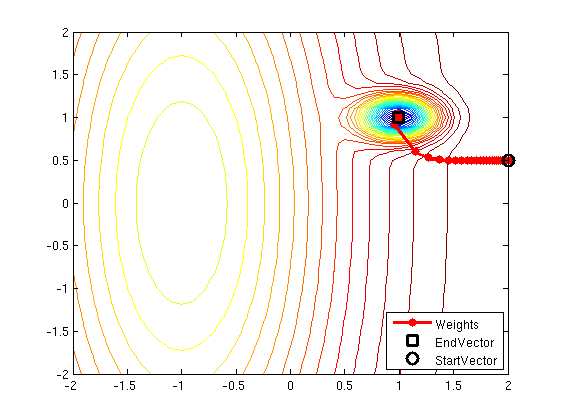
\includegraphics[width=0.8\textwidth]{./figures/213/path_w01_eta02.png}
  \caption{Verlauf von $\vect{w}$}
  \label{fig:213_path_w01_eta02}
\end{figure}

\begin{figure}[h!]
  \centering
  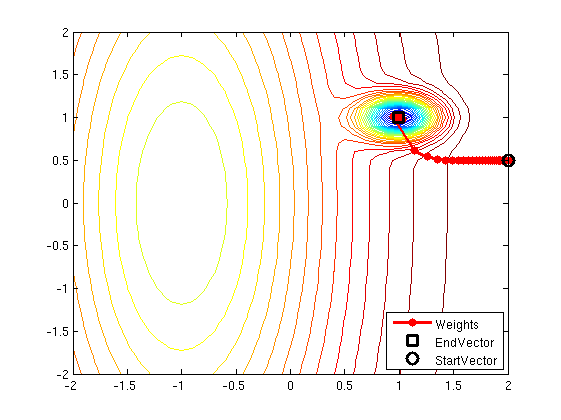
\includegraphics[width=0.8\textwidth]{./figures/213/path_w01_eta015.png}
  \caption{Verlauf von $\vect{w}$}
  \label{fig:213_path_w01_eta015}
\end{figure}

\begin{figure}[h!]
  \centering
  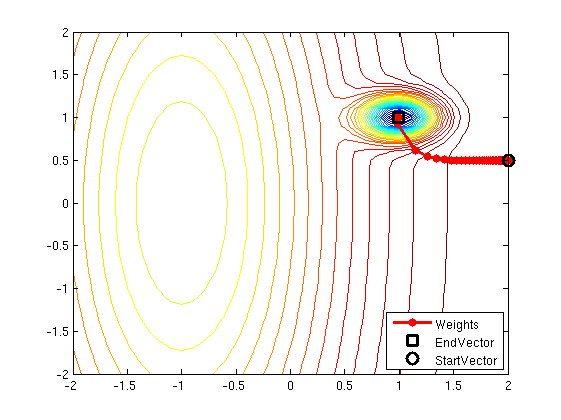
\includegraphics[width=0.8\textwidth]{./figures/213/path_w01_eta01.png}
  \caption{Verlauf von $\vect{w}$}
  \label{fig:213_path_w01_eta01}
\end{figure}

\begin{figure}[h!]
  \centering
  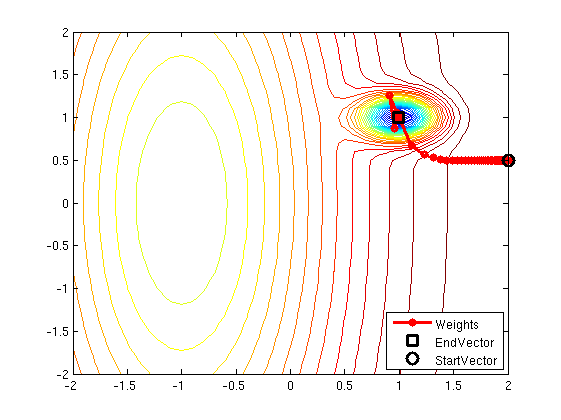
\includegraphics[width=0.8\textwidth]{./figures/213/path_w01_eta005.png}
  \caption{Verlauf von $\vect{w}$}
  \label{fig:213_path_w01_eta005}
\end{figure}

\begin{figure}[h!]
  \centering
  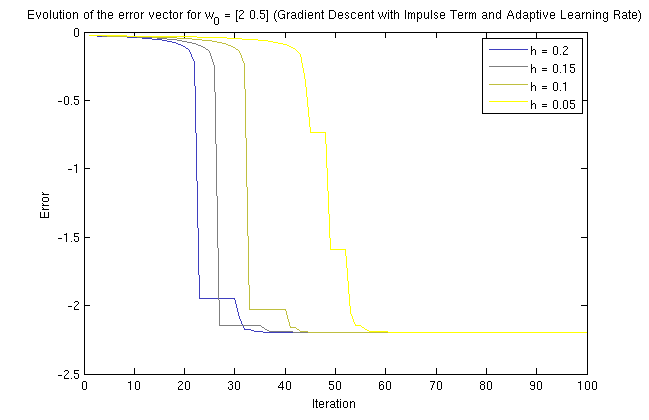
\includegraphics[width=0.8\textwidth]{./figures/213/error_w01.png}
  \caption{Verlauf von $f(\vect{w})$}
  \label{fig:213_error_w01}
\end{figure}

\begin{figure}[h!]
  \centering
  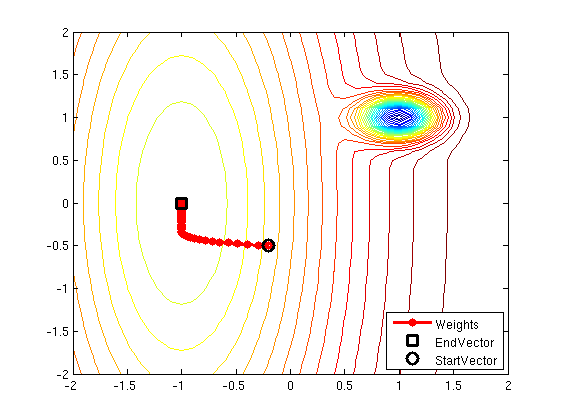
\includegraphics[width=0.8\textwidth]{./figures/213/path_w02_eta02.png}
  \caption{Verlauf von $\vect{w}$}
  \label{fig:213_path_w02_eta02}
\end{figure}

\begin{figure}[h!]
  \centering
  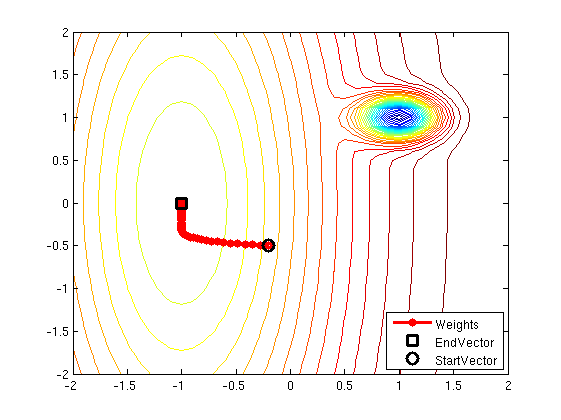
\includegraphics[width=0.8\textwidth]{./figures/213/path_w02_eta015.png}
  \caption{Verlauf von $\vect{w}$}
  \label{fig:213_path_w02_eta015}
\end{figure}

\begin{figure}[h!]
  \centering
  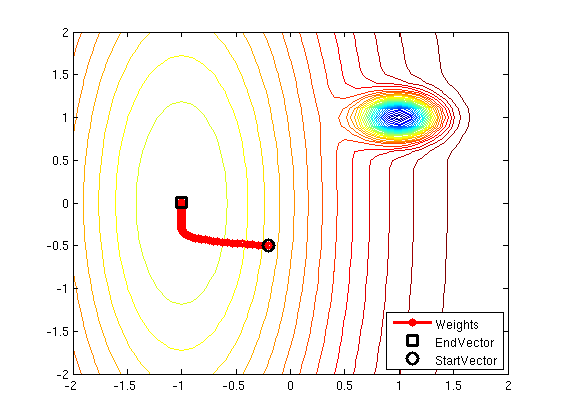
\includegraphics[width=0.8\textwidth]{./figures/213/path_w02_eta01.png}
  \caption{Verlauf von $\vect{w}$}
  \label{fig:213_path_w02_eta01}
\end{figure}

\begin{figure}[h!]
  \centering
  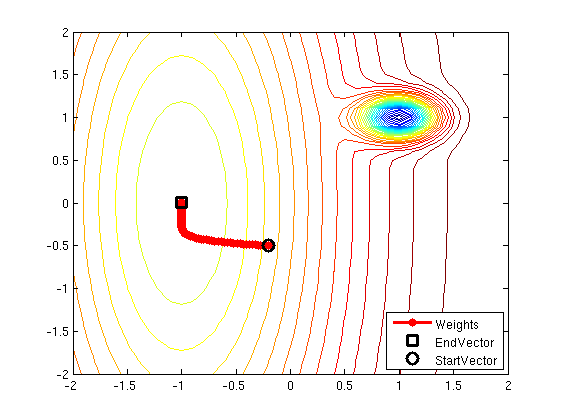
\includegraphics[width=0.8\textwidth]{./figures/213/path_w02_eta005.png}
  \caption{Verlauf von $\vect{w}$}
  \label{fig:213_path_w02_eta005}
\end{figure}

\begin{figure}[h!]
  \centering
  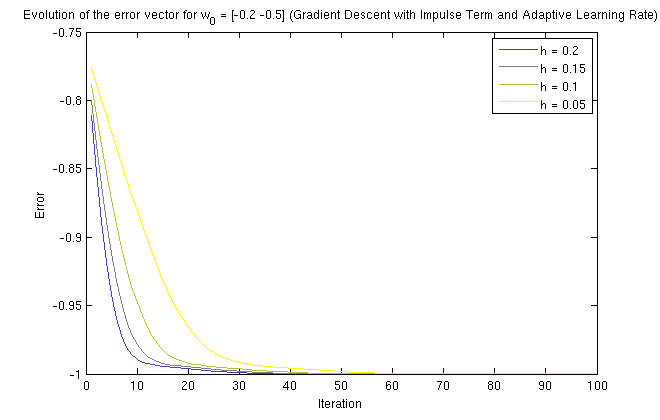
\includegraphics[width=0.8\textwidth]{./figures/213/error_w02.png}
  \caption{Verlauf von $f(\vect{w})$}
  \label{fig:213_error_w02}
\end{figure}

\clearpage

